
\documentclass[11pt,a4paper]{article}

% ==============================
% 📦 PACKAGES
% ==============================

\usepackage[utf8]{inputenc}
\usepackage[T1]{fontenc}
\usepackage{lmodern}
\usepackage{geometry}
\usepackage{amsmath, amssymb, amsthm}
\usepackage{mathtools}
\usepackage{graphicx}
\usepackage{float}
\usepackage{booktabs}
\usepackage{array}
\usepackage{enumitem}
\usepackage{xcolor}
\usepackage{hyperref}
\usepackage{tikz}
\usepackage{pgfplots}
\usepackage{listings}
\usepackage{tcolorbox}
\usepackage{tikz}
\usepackage[american]{circuitikz}
\pgfplotsset{compat=1.18}

% ==============================
% 📐 PAGE STYLE
% ==============================

\geometry{
    left=2.5cm,
    right=2.5cm,
    top=2.5cm,
    bottom=2.5cm
}

\setlength{\parindent}{0pt}
\setlength{\parskip}{6pt}

% ==============================
% 🎨 COLOR PALETTE (Minimal & Elegant)
% ==============================

\definecolor{mainblue}{RGB}{25,55,109}
\definecolor{lightgray}{RGB}{245,245,245}

% ==============================
% 📦 THEOREM ENVIRONMENTS
% ==============================

\newtheorem{theorem}{Teorema}[section]
\newtheorem{definition}{Definizione}[section]
\newtheorem{proposition}{Proposizione}[section]
\newtheorem{example}{Esempio}[section]

% ==============================
% 🧠 CUSTOM BOXES (Very Clean)
% ==============================

\newtcolorbox{importantbox}{
    colback=lightgray,
    colframe=mainblue,
    boxrule=0.8pt,
    arc=4pt
}

% ==============================
% 💻 CODE STYLE
% ==============================

\lstset{
    language=C++, % cambia se vuoi (Python, Java, ecc.)
    basicstyle=\ttfamily\small,
    keywordstyle=\color{blue},
    commentstyle=\color{gray},
    stringstyle=\color{red},
    numbers=left,
    numberstyle=\tiny,
    stepnumber=1,
    numbersep=8pt,
    backgroundcolor=\color{lightgray},
    frame=single,
    breaklines=true
}

% ==============================
% 📄 DOCUMENT
% ==============================

\begin{document}
% ==============================
\section{lezione del 20-03-26}
\subsection{Diodio Zener: Operare nel Breakdown}\label{sub:Diodio Zener: Operare nel Breakdown} % (fold)
Analizziamo un semplice circuto che utilizza il diodo zener.
\begin{center}
\begin{circuitikz}[american]
    % Disegno del loop principale
    \draw (0,0) node[ground] {}
        to[battery2, l=$V_2$, invert] (0,3)           % Generatore di tensione
        to[R, l=$R$] (3,3)                    % Resistenza
        to[short, -o] (3,2.5) node[right] {A}; % Nodo Anodo

    % Diodo Zener (invertito per mostrare la conduzione Zener)
    \draw (3,2.5) to[zD, invert] (3,0.5);

    % Chiusura del circuito
    \draw (3,0.5) node[right] {K}             % Nodo Catodo
        to[short, o-] (3,0)
        to (0,0);

    % Annotazioni in ROSSO (Corrente ID e Tensione VD)
    % Freccia della corrente ID
    \draw[red, thick, ->] (2.3, 0.7) -- (2.3, 2.3) 
        node[midway, left] {$I_D$};
    
    % Polarità e etichetta VD
    \node[red, font=\Large] at (3.8, 1.5) {$V_D$};
    \node[red, font=\Large] at (3.8, 2.6) {$-$};
    \node[red, font=\Large] at (3.8, 0.4) {$+$};

\end{circuitikz}
\end{center}
Risolvendo con la seconda legge di Kirchhoff alle maglie otteniamo l'equazione
\[
    -I_DR - V_2 - V_D = 0, \quad -V_2-  V_D = RI_D, \quad -\frac{V_2 + V_D}{R} = I_D
\]
Dalla quale abbiamo ottenuto l'equazione della \textit{retta di carico}
\[
    I_D = -\frac{V_2 + V_D}{R}
\]
In genere si indica con $I_Z = -I_D$ per facilitare l'analisi
% subsection Diodio Zener: Operare nel Breakdown (end)
\subsubsection{Regolatore di tensione con diodo zener}\label{sub:Regolatore di tensione con diodo zener} % (fold)
\begin{center}
    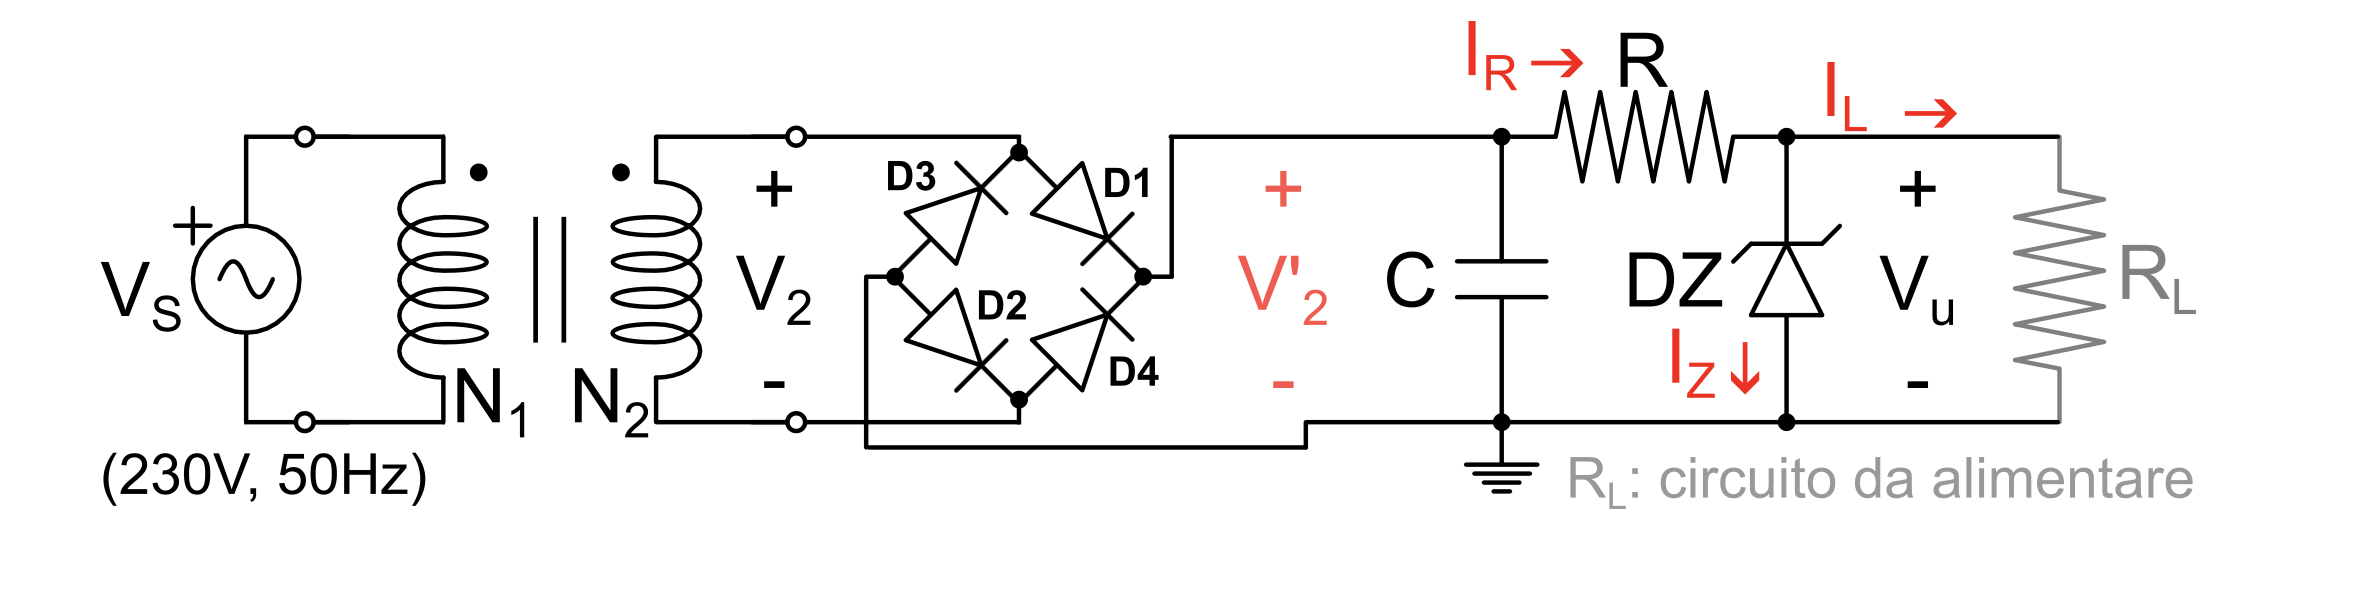
\includegraphics[scale=0.35]{../images/regolatore_di_tensione_diodo_zener.png}
\end{center}
Notiamo che se $I_Z > 0$ allora $V_u = V_Z$ possiamo quindi dire che:
\[
    I_R = \frac{V_2^{\prime} - V_Z}{R}, \quad I_L = \frac{V_Z}{R_L} ,\quad I_Z = I_R - I_L = \frac{V_2^{\prime} - V_Z}{R} - \frac{V_Z}{R_L} > 0
\]
Il fatto che $I_Z > 0$ ci assicurac che il diodo di zener sia in conduzione. \\
Mettiamo nella situazione di un progettista che deve scegliere il valore della resistenza $R$. 
Come decido il valore?
\begin{itemize}
    \item La tensione dopo il ponte di Greatz è soggeta a \textit{ripple}: $V_{2, \text{min}}' = \leq V_2 \leq V_{2, \text{max}}'$
    \item Quando il carico non richede corrente $(R \to +\infty)$ si che $I_L = 0$ quindi $I_Z = I_R$. 
            Da questo otteniamo 
            \[
                I_{Z,\text{max}} = \frac{V_{2,\text{max}}' - V_Z}{R}
            \]
            quindi 
            \[
                V_Z I_{Z,\text{max}} < P_{Z, \text{max}} \implies I_{Z, \text{max}} < \frac{P_{Z, \text{max}}}{V_Z} \implies R > \frac{(V_{2,\text{max}}' - V_Z)V_Z}{P_{Z, \text{max}}}
            \]
\end{itemize}
Il valore trovato è il valore \textbf{minimo tollerabile} di $R$ per il quale il circuito continua a funzionare come ci aspetteremmo.
% subsubsection Regolatore di tensione con diodo zener (end)
\subsection{Modello del diodio per piccolo segnali}\label{sub:Modello del diodio per piccolo segnali} % (fold)
Abbiamo già visto come comportarci in circuiti con diodio a grandi segnali. Oggi vogliamo focalizzarci
sull'aspetto duale che sono i \textbf{piccoli segnali}. Vediamo quindi quali approssimazione possiamo fare 
per risolvere circuiti di questo tipo.
\begin{center}
    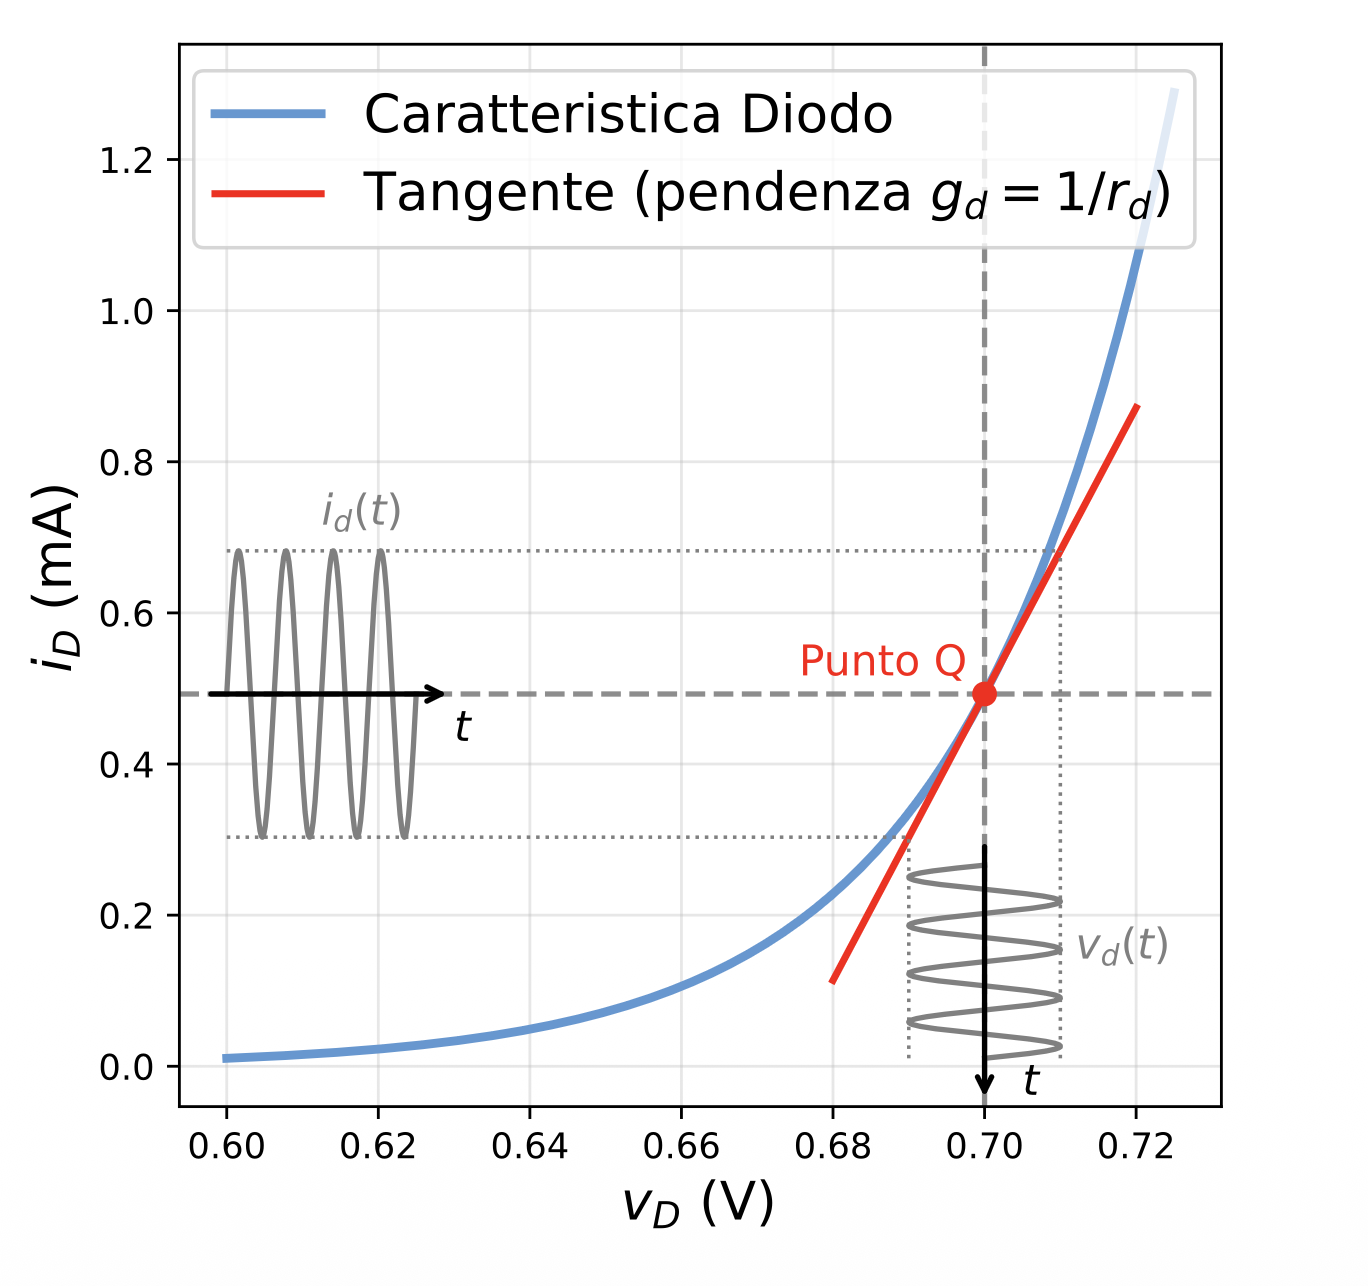
\includegraphics[scale=0.35]{../images/grafico_diodo_piccoli_segnali.png} 
\end{center}
Prestiamo importanza come già fatto in precedenta al punto $Q$ detto \textit{punto di riposo} di coordinate ($V_{DQ}, I{DQ}$). 
L'idea chiave è quella di dire che se le variazioni del segnale sono sufficientemente piccole rispetto alla tensione termica
che la curva esponenziale del diodo può essere approssimata con un segmento rettilineo tangente al punto $Q$. 
Queste semplificazione vengono adottate perchè portano a vantaggi: 
\begin{itemize}
    \item \textbf{Semplificazione}: vogliamo  evitare di risolvere equazioni trascendentali ma lineari trattando il diodo come una semplice resistenza $r_d$. 
    \item \textbf{Sovrapposizione degli effetti}: un circuito \textit{linerarizzato} può essere studiato con il 
\textit{principio di sovrapposizione degli effetti}, possiamo quindi separare l'analisi in \textbf{continua} (che fissa il punto $Q$) dall'analisi 
\textbf{alternata} (che elabora il segnale).
\item \textbf{Linerarizzazione}: se $|v_d(t)| << V_{DQ}:$ 
    \[
        i_D(t) = f(V_{DQ}) + \left . \frac{\partial f}{\partial v_D)} \right |_{V_{DQ}}\cdot v_D(t) \leftrightarrow i_D(t) =I_{DQ} + i_d(t)
    \]
    \[
        \implies I_{DQ} = f(V_{DQ}), \quad i_d(t) = \left . \frac{\partial f}{\partial V_D} \right |_{V_{DQ}} \cdot v_D(t)
    \]
\end{itemize}
Abbiamo quindi che 
\begin{itemize}
    \item  \textbf{Conduttanza differenziale}: 
        \[
            g_d = \frac{i_d}{v_d} = \left . \frac{\partial f}{\partial V_D} \right |_{V_{DQ}}
        \]
    \item \textbf{Resistenza differenziale}: 
        \[
            r_d = \frac{1}{g_d} = \left( \left . \frac{\partial f}{\partial V_D} \right |_{V_{DQ}} \right )^{-1}
        \]
\end{itemize}
Analiticamente possiamo dire 
\[
    i_D = f(v_D) = I_S(e^{\frac{V_{DQ}}{\eta V_T}} - 1)
\]
mettendo tutto insieme otteniamo
\[
    g_d = \left. \frac{\partial f}{\partial V_D} \right|_{V_{DQ}} = \frac{1}{\eta V_T} I_S e^{\frac{V_{DQ}}{\eta V_T}} = \frac{I_S \left(e^{\frac{V_{DQ}}{\eta V_T}} - 1\right) + I_S}{\eta V_T} \approx \frac{I_{DQ}}{\eta V_T}, \quad I_{DQ} \gg I_S
\]
Notiamo che i \textit{parametri differenziali} dipendono dal punto di riposo ($V_{DQ}$).
% subsection Modello del diodio per piccolo segnali (end)
\end{document}

